\chapter{\IfLanguageName{dutch}{Stand van zaken}{State of the art}}%
\label{ch:stand-van-zaken}

% Tip: Begin elk hoofdstuk met een paragraaf inleiding die beschrijft hoe
% dit hoofdstuk past binnen het geheel van de bachelorproef. Geef in het
% bijzonder aan wat de link is met het vorige en volgende hoofdstuk.

% Pas na deze inleidende paragraaf komt de eerste sectiehoofding.

%Dit hoofdstuk bevat je literatuurstudie. De inhoud gaat verder op de inleiding, maar zal het onderwerp van de bachelorproef *diepgaand* uitspitten. De bedoeling is dat de lezer na lezing van dit hoofdstuk helemaal op de hoogte is van de huidige stand van zaken (state-of-the-art) in het onderzoeksdomein. Iemand die niet vertrouwd is met het onderwerp, weet nu voldoende om de rest van het verhaal te kunnen volgen, zonder dat die er nog andere informatie moet over opzoeken \autocite{Pollefliet2011}.
%
%Je verwijst bij elke bewering die je doet, vakterm die je introduceert, enz.\ naar je bronnen. In \LaTeX{} kan dat met het commando \texttt{$\backslash${textcite\{\}}} of \texttt{$\backslash${autocite\{\}}}. Als argument van het commando geef je de ``sleutel'' van een ``record'' in een bibliografische databank in het Bib\LaTeX{}-formaat (een tekstbestand). Als je expliciet naar de auteur verwijst in de zin, gebruik je \texttt{$\backslash${}textcite\{\}}.
%Soms wil je de auteur niet expliciet vernoemen, dan gebruik je \texttt{$\backslash${}autocite\{\}}. In de volgende paragraaf een voorbeeld van elk.
%
%\textcite{Knuth1998} schreef een van de standaardwerken over sorteer- en zoekalgoritmen. Experten zijn het erover eens dat cloud computing een interessante opportuniteit vormen, zowel voor gebruikers als voor dienstverleners op vlak van informatietechnologie~\autocite{Creeger2009}.

In dit gedeelte van de scriptie zal de huidige manier van asset tracking binnenin de bouwindustrie beschreven worden. Bluetooth Low Energy en de werking ervan zal ook uitvoerig worden besproken samen met de verschillen tussen BLE en het klassieke Bluetooth. Verder zal er verklaard worden hoe Bluetooth Low Energy bij smartphones werkt. Secutiry?

\subsection{Asset tracking in de bouwindustrie}

Het lokaliseren van middelen op een bouwterrein is in het verleden altijd een uitdagende taak geweest. Onbenutte middelen zoals werkgereedschap of machines zouden tot de grote meerderheid van verspilling in de bouwindustrie bijdragen \autocite{Nasr2013}. Door het gebruik van verschillende technologieën hebben onderzoekers zich gericht tot het ontwikkelen van plaatsbepalingssystemen als poging om dit probleem aan te pakken. Met behulp van deze systemen kan activa zoals werkgereedschap, machines of personeel gevolgd worden met onder andere als doel op deze manier hun veiligheid te bewaren.\\

De meest technologieën die het meest gebruikt worden voor asset tracking in de bouwindustrie zijn GPS, RFID en UWD.

\subsubsection{Global Positioning System}

Het Global Positioning System (GPS) is een positionering en navigatie systeem ontwikkeld door de Amerikaans ministerie van defensie \autocite{McNeff} in de jaren zestig. Het bestaat ondertussen uit meer dan dertig satellieten die rond onze aarde cirkelen. Deze kunnen met behulp van de atomische klok die elke satelliet aan boord heeft en hun gekende precieze locatie continu signalen uitzenden die gebruikers op aarde kunnen ontvangen. Hiermee is het mogelijk de tijd en locatie van de gebruiker te bepalen met respectievelijk een paar nanoseconden en meter speling. Elke GPS-satelliet kent zijn eigen baanlocatie en systeemtijd. Om de positie van een ontvanger nauwkeurig te kunnen bepalen moeten er ten te allen tijde minstens vier satellieten zichtbaar zijn die voldoende van elkaar gescheiden zijn. Met behulp van trilateratie, wat de basis is van de gebruikte technieken waarbij de afstandsmetingen van \(n + 1\) satellieten worden gebruikt voor een n-dimensionale positiebepaling \autocite{Rahman2012} is het mogelijk de positie te bepalen van een gebruiker op aarde. Hier zal niet verder op uitgebreid worden want dit is niet het doel van deze scriptie.\\

Nu nog ivm de bouwindustrie...

NOG EEN FIGUURTJE?

\subsubsection{Radio Frequenty Identifier}

Radio Frequenty Identifier (RFID)  is een draadloze communicatietechnologie die in zijn simpelste vorm objecten kan detecteren, opsporen, identificeren, volgen en controleren \autocite{Tan2022}. Het bestaat voornamelijk uit drie elementen, readers, antennes en tags. De reader of soms ook transeiver genaamd heeft de mogelijkheid radio frequentie (RF) elektrische golven te sturen naar een of meerdere RFID tags. De tags hoeven dus niet in het gezichtsveld van de reader te zitten. Deze tags (actief of passief) ontvangen de elektrische golf met hun antenne en zetten deze met behulp van een spoel om naar elektrische stroom. Vervolgens wordt deze stroom door de tag die bevestigd is aan een fysiek object gebruikt om terug via een RF elektrische golf een antwoord te sturen naar de reader.\\

RFID tags kunnen opgedeeld worden in drie soorten. Actieve, semi-passief en passieve tags \autocite{Mezzanotte2021}.  Actieve tags bezitten een batterij die heel het systeem van stroom voorziet. Zo een systeem van een actieve tag bestaat uit een ontvanger, een zender en omgevingssensoren. Het principe van een passieve tag is vrij verschillende want deze tags zullen de stroom die toekomst als RF elektrische golf omgezet wordt door de ingebouwde spoel gebruiken om een antwoord te verzenden. Passieve tags hebben geen batterij en transmitter. Semi-passieve tags zijn een mix van actief en passief in de zin dat ze dezelfde functioneringsprincipe gebruiken maar ze hebben wel een batterij om de microchip of sensoren van stroom te voorzien.\\

RFID wordt vaak gebruikt in sectoren waar er bijvoorbeeld producten worden gestockeerd in een magazijn. Indien er door een reader een vraagimpuls wordt verzonden kunnen de tags antwoorden met een digitaal gegeven. Dit is vaak hun identificatienummer. Op deze manier kan zo een ID worden toegewezen aan ieder product bij het printen van de tag en kan een magazijnmedewerker met gebruik van een reader op deze manier het juiste product vinden in een magazijn.\\

In de bouwindustrie wordt dit op een gelijkaardige manier gebruikt om assets te traceren en lokaliseren.

\subsubsection{Ultra-wideband}


\subsection{Bluetooth Low Energy}
Ook wel Bluetooth Smart genoemd, Bluetooth Low Energy is een wireless personal area network (PAN). Ontworpen en ontwikkeld door de Bluetooth Special Interest Group (SIG). Dit is het non-profit normalisatie-instituut die toezicht houdt op de ontwikkeling van Bluetooth standaarden en het in licentie geven van de Bluetooth-technologieën en -handelsmerken aan fabrikanten. \\

BLE zendt gegevens uit via 40 kanalen in de 2.4GHz ISM-frequentieband \autocite{Kumbhar_2017}. Dit is een gedeelte van het radiospectrum gereserveerd voor industriele (Industrial), wetenschappelijke (Scientific) en medische (Medical) doeleinden zoals microgolven, medische apparatuur, procesverwarming en soorten elektrolampen. De laatste jaren zijn er ook draadloze communicatie toestellen geproduceerd die ook deze banden kunnen gebruiken zonder storing te veroorzaken voor bestaande apparaten die gebruik maken van de ISM-banden, zoals BLE.\\

Vergeleken met Bluetooth Classic ondersteunt Bluetooth Low Energy meerdere communicatietopologieën, namelijk point-to-point, mesh en broadcast. Terwijl Bluetooth Classic enkel point-to-point ondersteunt. Door de mesh topologie kunnen er grootschalige en betrouwbare netwerken gebouwd worden tussen verschillende toestellen. Hoewel Bluetooth vroeger meer bekend stond voor gegevens uitwissen tussen toestellen wordt het tegenwoordig ook vaak gebruikt voor het positioneren van apparaten. Dit wordt gedaan aan de hand van een paar concepten.

\subsubsection{Real-Time Locating System}

Een Real-Time Locating System heeft als hoofddoel het identificeren en real-time de positie of hoek van bepaalde objecten te kunnen bepalen \autocite{Lehtimaki2018}, in dit geval gebruik makend van radio golven maar nog mogelijkheden zijn infrarood of ultrasound. Dit is meestal in een gebouw of een ander afgebakend gebied. Dit is van toepassing op bijvoorbeeld de locatie bepalen van assets of mensen en nog zeer veel IoT (Internet of Things) toepassingen.

\subsubsection{Angle of Arrival}

Bluetooth maakt gebruik van twee verschillende methoden om de locatie, specifiek de afstand en richting van een Bluetooth Low Energy signaal te bepalen. Angle of Arrival is hier een van. 
In deze methode zend een apparaat zoals een asset tag met behulp van een antenne een signaal uit. Deze wordt opgevangen door een ontvangend apparaat die over een reeks antennes beschikt. Hierdoor kan het ontvangend gegevens verzamelen waarmee de richting van het signaal berekend kan worden. Theoretisch gezien zullen de ontvangende reeks antennes faseverschillen zien door de verschillende afstanden tot de zender maar dit is net zoals de meeste zaken in de praktijk niet zo simpel.
\subsubsection{Angle of Departure}

Het fundamentele idee van Angle of Depature is hetzelfde als die van Angle of Arrival maar nu zijn de rollen omgedraaid. Het apparaat dat een signaal ontvangt heeft maar een antenne en degene dat de data verzend heeft er meerdere. Dit kan u zien op figuur \ref{fig:aop} waarbij TX de zender is en RX de ontvanger. Bij Angle of Departure berekent het ontvangende apparaat zelf zijn locatie aan de hand van de verschillende antennes van het zendende apparaat en hun posities.\\

Hier kunnen veel combinaties in gemaakt worden en met behulp van de Received Signal Strength Indicator (RSSI) zijn er nog eens extra mogelijkheden.

%\begin{figure}
%    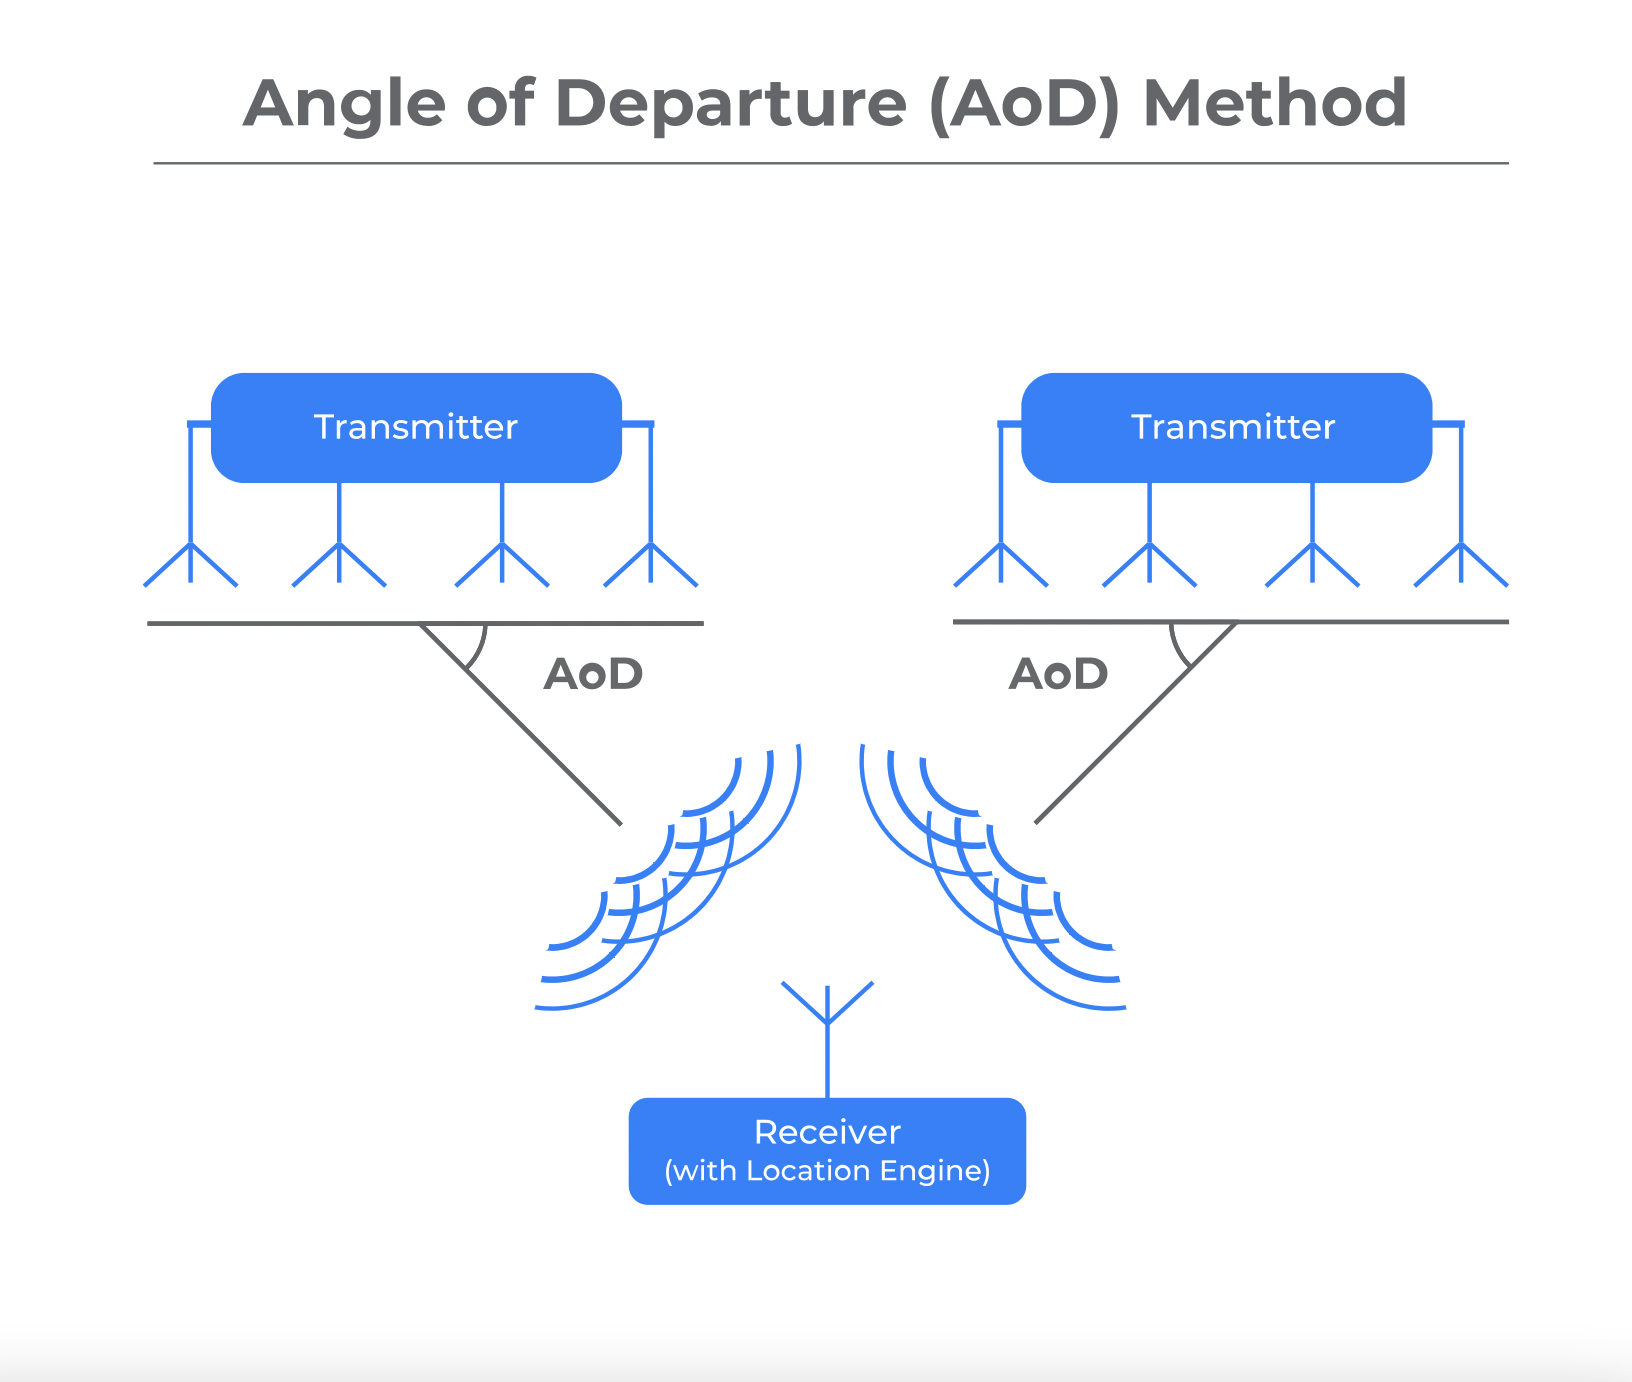
\includegraphics[width=\linewidth]{angle_of_departure_graphic.png}
%    \caption{Angle of Departure}
%    \label{fig:aop}
%\end{figure}

\subsubsection{Received Signal Strength Indicator}

De Received Signal Strength Indicator (RSSI)

\subsection{Smartphones}

Hoe werkt BLE bij smartphone?

Smartphones doen dit aan de hand van RSS \autocite{Chen2017}.


\subsection{Hoe veilig is Bluetooth Low Energy?}
